\documentclass{beamer}

\usepackage{ctex}
\usepackage{braket}
\usepackage{graphicx}
\graphicspath{{pics/}}
\usepackage{subcaption}  %插入子图用
\usepackage{booktabs}
\usepackage{amsmath} % 提供 \xrightarrow 等命令

\setbeamertemplate{caption}[numbered]  %让插入的图片自动编号(beamer默认不编号)
\usefonttheme{serif}   %在公式中使用使用标准的Latex字体(有衬线的字体),区分小的L和大写的I
%beamer中默认使用Sans Serif字体,即没有衬线的字体
\renewcommand{\thefootnote}{}    %取消脚注的编号,在后面花括号内添加其他符号也可改变脚注符号
\usepackage{caption}
\usepackage[english]{babel} % 将时间改成英
\usepackage{calligra}
\setbeamertemplate{navigation symbols}

% 修改beamer脚注的默认设置
\usepackage{etoolbox}  % 引入etoolbox以方便进行宏的修补
\makeatletter
\defbeamertemplate*{footnote}{nonumber}{
	\parindent 1em\noindent% 
	\raggedright
	\insertfootnotetext\par
}
\setbeamertemplate{footnote}[nonumber]  % 应用自定义的脚注模板
\makeatother

% 幻灯片字体和主题
\usepackage{times}
\usetheme{CambridgeUS}
\usecolortheme{dolphin}

% HITsz校徽,badge文件为校徽
\pgfdeclareimage[height=0.6cm]{badge}{badge}
\logo{\pgfuseimage{badge}}

% 目录设置
\AtBeginSection[]{
	\begin{frame}
		\tableofcontents[currentsection]
	\end{frame}
}

% 首页信息
\title[毕业设计答辩]
{轮足机器人控制系统设计}

\author[晋禾木]
{\fontsize{8}{10}\selectfont
	晋禾木
	\\[10pt]
	 指导老师:陈晓侠
	 \\[10pt]
	\href{mailto:490754775@qq.com}
	{Email: \textit{490754775@qq.com}}}

\institute[电气工程学院]
{\fontsize{8}{10}\selectfont
	大连交通大学电气工程学院}

% \date[\today]
\date[June 17, 2025]
{\fontsize{8}{10}
	\selectfont June 17, 2025}

% 正文
\begin{document}
	\logo{}
	\begin{frame}
		\titlepage
		\begin{center}
			\vspace{-15pt}
			\includegraphics[width=0.3\linewidth]{Badge.png}
		\end{center}
	\end{frame}
	
	% 目录
	\logo{\pgfuseimage{badge}}
	\begin{frame}
		\frametitle{Contents}
		\tableofcontents
	\end{frame}
	\logo{}
	
	
	
	
	
	% Section 1
	\section[研究背景和意义]{研究背景和意义}


	\begin{frame}{研究背景}
		\begin{figure}[t]
			\centering
			\begin{subfigure}{0.3\textwidth}
				\centering
				\includegraphics[width=0.7\linewidth]{img/chapter1/3}
				\caption{轮式机器人}
			\end{subfigure}
			\hfill
			\begin{subfigure}{0.3\textwidth}
				\centering
				\includegraphics[width=1.2\linewidth]{img/chapter1/4}
				\caption{足式机器人}
			\end{subfigure}
			\hfill
			\begin{subfigure}{0.3\textwidth}
				\centering
				\includegraphics[width=0.7\linewidth]{img/chapter1/1}
				\caption{轮足机器人}
			\end{subfigure}
			\captionsetup{font=scriptsize} 
			\caption{机器人示意图} 
		\end{figure}
		\begin{itemize}
			\item 传统轮式机器人移动速度快,但难以应对复杂地形。
			\item 足式机器人具有强地形适应能力,但运动效率较低。
			\item 轮足机器人融合两者优势,兼具速度与机动性。

		\end{itemize}
	\end{frame}
	
	\begin{frame}{研究意义}
		\begin{figure}          
			\centering              
			\includegraphics[width=0.4\linewidth]{img/chapter1/2}  
			\captionsetup{font=scriptsize} 
			\caption{五连杆轮足机器人} 
		\end{figure}  
		\begin{itemize}
			\item 近年来在灾害搜救、野外巡检、军事侦察等领域获得广泛关注。
			\item 实现软硬件一体化设计,提升轮足机器人的实用性与工程可部署性。
			\item 为后续复杂环境中机器人应用提供参考与技术支撑。
		\end{itemize}
	\end{frame}

	
	

	

	
	
	
	
	% Section 2
	\section[系统总体设计]{系统总体设计}

	\begin{frame}
		\frametitle{总体方案框架}
		\begin{figure}          
			\centering              
			\includegraphics[width=3.8in]{img/chapter2/1.pdf}  
			\captionsetup{font=scriptsize} 
			\caption{总体框架图} 
		\end{figure}               
	\end{frame}
	
	\begin{frame}
		\frametitle{元件选型}
		\begin{figure}[t]
			\centering
			\begin{subfigure}{0.45\textwidth}
				\centering
				\includegraphics[width=0.5\linewidth]{img/chapter2/2}
				\caption{STM32H723VET6开发板}
			\end{subfigure}
			\hfill
			\begin{subfigure}{0.45\textwidth}
				\centering
				\includegraphics[width=0.5\linewidth]{img/chapter2/3}
				\caption{DM-J4310关节电机}
			\end{subfigure}
			
			\begin{subfigure}{0.45\textwidth}
				\centering
				\includegraphics[width=0.5\linewidth]{img/chapter2/4}
				\caption{DM-H6215轮毂电机}
			\end{subfigure}
			\captionsetup{font=scriptsize} 
			\caption{元件选型}
		\end{figure}
	\end{frame}


	\begin{frame}
	\frametitle{结构设计}
			\begin{figure}          
			\centering              
			\includegraphics[width=3.8in]{img/chapter2/6}  
			\captionsetup{font=scriptsize} 
			\caption{整体结构图} 
		\end{figure}  
	\end{frame}	
	
		\begin{frame}
		\frametitle{结构设计}
		\begin{figure}          
			\centering              
			\includegraphics[width=3.8in]{img/chapter2/7.pdf}  
			\captionsetup{font=scriptsize} 
			\caption{内部结构图} 
		\end{figure}  
	\end{frame}	
	
			\begin{frame}
		\frametitle{结构设计}
		\begin{figure}          
			\centering              
			\includegraphics[width=3.8in]{img/chapter2/8}  
			\captionsetup{font=scriptsize} 
			\caption{腿部结构图} 
		\end{figure}  
	\end{frame}	
	
	% Section 3
	\section[控制策略与仿真]{控制策略与仿真}
	\begin{frame}
		\frametitle{系统建模}
		\begin{figure}         
			%\centering              
			\includegraphics[width=0.33\linewidth]{img/chapter3/1.pdf}  
			\captionsetup{font=scriptsize} 
			\caption{倒立摆示意图} 
			
		\end{figure}  
	\end{frame}
	
	\begin{frame}{模型参数}
		\scriptsize % 控制整体字体大小
		\centering
		\begin{tabular}{cccc}
			\toprule
			\textbf{符号} & \textbf{含义} & \textbf{正方向} & \textbf{单位} \\
			\midrule
			$\theta$  & 摆杆与竖直方向夹角         & 图示为正   & rad \\
			$x$       & 驱动轮位移                 & 箭头所示   & m \\
			$\phi$    & 机体与水平夹角             & 图示为正   & rad \\
			$T$       & 驱动轮输出力矩             & 同 $\theta$ & N·m \\
			$T_p$     & 髋关节输出力矩             & 同 $\alpha$ & N·m \\
			$N$       & 驱动轮对摆杆水平力         & 箭头所示   & N \\
			$P$       & 驱动轮对摆杆竖直力         & 箭头所示   & N \\
			$N_M$     & 摆杆对机体水平方向分量     & 箭头所示   & N \\
			$P_M$     & 摆杆对机体竖直方向分量     & 箭头所示   & N \\
			$N_f$     & 地面对驱动轮摩擦力         & 箭头所示   & N \\
			$R$       & 驱动轮半径                 & 无         & m \\
			$L$       & 摆杆重心到驱动轮轴距离     & 无         & m \\
			$L_M$     & 摆杆重心到机体转轴距离     & 无         & m \\
			$l$       & 机体重心到其转轴距离       & 无         & m \\
			$m_w$     & 驱动轮转子质量             & 无         & kg \\
			$m_p$     & 摆杆质量                   & 无         & kg \\
			$M$       & 机体质量                   & 无         & kg \\
			$I_w$     & 驱动轮转子转动惯量         & 无         & kg·m$^2$ \\
			$I_p$     & 摆杆绕质心转动惯量         & 无         & kg·m$^2$ \\
			$I_M$     & 机体绕质心转动惯量         & 无         & kg·m$^2$ \\
			\bottomrule
		\end{tabular}
	\end{frame}
	
	
	
	\begin{frame}
		\frametitle{力学分析}
		对于驱动轮,有:
		\begin{align*}
			m_w \ddot{x} &= N_f - N \tag{3-1} \\
			I_w \frac{\ddot{x}}{R} &= T - N_f R \tag{3-2}
		\end{align*}
		合并上述两式并消去 $N_f$ 得到 $\ddot{x}$ 的表达式:
		\begin{equation*}
			\ddot{x} = \frac{T - N R}{I_w / R + m_w R} \tag{3-3}
		\end{equation*}
	\end{frame}
	
	\begin{frame}
		\frametitle{力学分析}
		对于摆杆,有:
		\begin{gather*}
			N - N_M = m_p \frac{\partial^2}{\partial t^2}(x + L \sin\theta) \\
			P - P_M - m_p g = m_p \frac{\partial^2}{\partial t^2} (L \cos\theta) \\
			I_p \ddot{\theta} = (P L + P_M L_M) \sin\theta - (N L + N_M L_M) \cos\theta - T + T_p
		\end{gather*}
		
		对于机体,有:
		\begin{gather*}
			N_M = M \frac{\partial^2}{\partial t^2} \left(x + (L + L_M) \sin\theta - l \sin\varphi\right) \\
			P_M - M g = M \frac{\partial^2}{\partial t^2} \left((L + L_M) \cos\theta + l \cos\varphi\right) \\
			I_M \ddot{\varphi} = T_p + N_M l \cos\varphi + P_M l \sin\varphi
		\end{gather*}
	\end{frame}

	
	\begin{frame}
		\frametitle{状态空间方程}
		由于系统是多输入、多输出的模型,可以采用状态空间方程来描述系统。首先定义状态向量 $\mathbf{x}$ 和控制向量 $\mathbf{u}$ 分别为:
		
		\[
		\mathbf{x} = \begin{bmatrix}
			\theta \\
			\dot{\theta} \\
			x \\
			\dot{x} \\
			\varphi \\
			\dot{\varphi}
		\end{bmatrix}
		\quad
		\mathbf{u} = \begin{bmatrix}
			T \\
			T_p
		\end{bmatrix}
		\]
		
		由于系统是非线性系统,无法直接使用线性状态空间方程表示与控制,因此需要将非线性系统线性化,再对其进行相应的控制处理。定义系统的非线性模型为:
		
		\[
		\dot{\mathbf{x}} = f(\mathbf{x}, \mathbf{u}) \tag{3-4}
		\]
	\end{frame}
	
	
	\begin{frame}
	\frametitle{状态空间方程}

		
		选定状态变量 $\mathbf{x}$ 与控制变量 $\mathbf{u}$,对系统在平衡工作点处进行线性化处理,求解相应的雅可比矩阵,用以构建线性状态空间模型:
		
		\[
		A = \left. \frac{\partial f}{\partial \mathbf{x}} \right|_{(\bar{\mathbf{x}}, \bar{\mathbf{u}})}, \quad
		B = \left. \frac{\partial f}{\partial \mathbf{u}} \right|_{(\bar{\mathbf{x}}, \bar{\mathbf{u}})}
		\]
		
		其中,$\bar{\mathbf{x}}, \bar{\mathbf{u}}$ 为系统平衡点,即满足 $f(\bar{\mathbf{x}}, \bar{\mathbf{u}}) = 0$ 的解:
		
		\[
		\bar{\mathbf{x}} = \begin{bmatrix}
			0 \\
			0 \\
			x \\
			0 \\
			0 \\
			0
		\end{bmatrix}, \quad
		\bar{\mathbf{u}} = \begin{bmatrix}
			0 \\
			0
		\end{bmatrix}
		\]
		
	\end{frame}
	
	\begin{frame}
		\frametitle{状态空间方程}
		将非线性系统转化为线性状态空间形式 $\dot{\mathbf{x}} = A\mathbf{x} + B\mathbf{u}$,可得:
		
		\[
		\dot{\mathbf{x}} =
		\begin{bmatrix}
			0 & 1 & 0 & 0 & 0 & 0 \\
			A_1 & 0 & A_2 & 0 & 0 & 0 \\
			0 & 0 & 0 & 1 & 0 & 0 \\
			A_3 & 0 & A_4 & 0 & 0 & 0 \\
			0 & 0 & 0 & 0 & 0 & 1 \\
			A_5 & 0 & A_6 & 0 & 0 & 0
		\end{bmatrix}
		\mathbf{x} +
		\begin{bmatrix}
			0 & 0 \\
			B_1 & B_2 \\
			0 & 0 \\
			B_3 & B_4 \\
			0 & 0 \\
			B_5 & B_6
		\end{bmatrix}
		\mathbf{u}
		\tag{3-5}
		\]
		
		系统输出向量定义为:
		
		\[
		\mathbf{y} = I_6 \mathbf{x} \tag{3-6}
		\]
		
		可控矩阵满秩,系统具备完全可观性。
		

	\end{frame}

		\begin{frame}
		\frametitle{LQR}
		依据现代最优控制理论,设计反馈控制律形式为:
		
		\[
		\mathbf{u} = -K \mathbf{x} \tag{3-7}
		\]
		即:
		\[
		\mathbf{u} = -
		\begin{bmatrix}
			k_{11} & k_{12} & k_{13} & k_{14} & k_{15} & k_{16} \\
			k_{21} & k_{22} & k_{23} & k_{24} & k_{25} & k_{26}
		\end{bmatrix}
		\begin{bmatrix}
			\theta \\
			\dot{\theta} \\
			x \\
			\dot{x} \\
			\varphi \\
			\dot{\varphi}
		\end{bmatrix}
		\tag{3-8}
		\]


		
	\end{frame}
	
	
	\begin{frame}
	\frametitle{LQR}
	为优化控制性能,引入线性二次型最优调节器(LQR)策略,通过构造如下性能指标函数:
	
	\[
	J = \int_{0}^{\infty} \left( \mathbf{x}^\top Q \mathbf{x} + \mathbf{u}^\top R \mathbf{u} \right) \, dt
	\tag{3-9}
	\]
	
	其中 $Q$、$R$ 为系统权重矩阵,分别反映系统状态与控制输入的惩罚程度。根据 LQR 理论,为最小化该性能指标函数,控制输入应满足:
	
	\[
	\mathbf{u} = -R^{-1} B^\top P \mathbf{x}
	\tag{3-10}
	\]
	
	由此,反馈矩阵 $K$ 可表示为:
	
	\[
	K = R^{-1} B^\top P
	\tag{3-11}
	\]
	
	其中 $P$ 是满足以下代数 Riccati 方程的对称正定矩阵:
	
	\[
	A^\top P + P A - P B R^{-1} B^\top P + Q = 0
	\tag{3-12}
	\]
			
	\end{frame}

	\begin{frame}
	\frametitle{LQR}
	为增强系统的运动跟踪能力,引入状态参考项 $\mathbf{x}_d$,将控制律拓展为:
	
	\[
	\mathbf{u} = K (\mathbf{x}_d - \mathbf{x}) 	\quad
	\mathbf{x}_d =
	\begin{bmatrix}
		0 \\
		0 \\
		\hat{x} \\
		\dot{\hat{x}} \\
		0 \\
		0
	\end{bmatrix}
	\]
	
	

	
	对矩阵各元素 $K_{ij}(L_0)$ 随腿长变化的规律进行三次多项式拟合:
	
	\[
	K_{ij}(L_0) = p0_{ij} + p1_{ij} L_0 + p2_{ij} L_0^2 + p3_{ij} L_0^3
	\]
	
	最终,可得机器人在纵向运动控制任务下的控制律表达式为:
	
	\[
	\mathbf{u} = K(L_0) \left( \mathbf{x}_d - \mathbf{x} \right)
	\]
	
	\end{frame}
	
	\begin{frame}
		\frametitle{K矩阵拟合}
		\begin{figure}          
			\centering
			\vspace{-150pt}             
			\includegraphics[width=\linewidth]{img/chapter3/data.pdf}  
			\captionsetup{font=scriptsize} 
			\vspace{-165pt} 
			\caption{K矩阵拟合示意图} 
			
		\end{figure}  
	\end{frame}

	\begin{frame}
	\frametitle{平面五连杆解算}
		\begin{figure}          
		\centering              
		\includegraphics[width=0.6\linewidth]{img/chapter3/2}  
		\captionsetup{font=scriptsize} 
		\caption{平面五连杆示意图} 
		
		\end{figure}  
	\end{frame}
	
	\begin{frame}
		\frametitle{平面五连杆解算}
		中间节点 $B$ 与 $D$ 的位置关系:
		\begin{equation*}
			\begin{cases}
				x_B + l_2 \cos\varphi_2 = x_D + l_3 \cos\varphi_3 \\
				y_B + l_2 \sin\varphi_2 = y_D + l_3 \sin\varphi_3
				\tag{3-14}
			\end{cases}
		\end{equation*}
		解方程组可推导出中间关节角度 $\varphi_2$ 的表达式:
		\begin{equation*}
			\varphi_2 = 2\arctan{\left(\frac{B_0 + \sqrt{A_0^2 + B_0^2 - C_0^2}}{A_0 + C_0}\right)}
		\end{equation*}
		其中:
		\begin{gather*}
			A_0 = 2l_2(x_D - x_B) \\
			B_0 = 2l_2(y_D - y_B) \\
			C_0= l_2^2 + l_{BD}^2 - l_3^2 \\
			l_{BD} = \sqrt{(x_D - x_B)^2 + (y_D - y_B)^2}
		\end{gather*}
		
	\end{frame}
	
	
	\begin{frame}
		\frametitle{平面五连杆解算}
			在计算出 $\varphi_2$ 后,可以进一步计算末端点 $C$ 的坐标:
			\begin{equation*}
				\begin{cases}
					x_C = l_1 \cos\varphi_1 + l_2 \cos\varphi_2 \\
					y_C = l_1 \sin\varphi_1 + l_2 \sin\varphi_2
				\end{cases}
			\end{equation*}
			
			再将末端位置转换为极坐标形式:
			\begin{align*}
				L_0 &= \sqrt{(x_C - l_5/2)^2 + y_C^2} \\
				\varphi_0 &= \arctan\left(\frac{y_C}{x_C - l_5/2}\right)
			\end{align*}
	\end{frame}
	
	
	\begin{frame}
		\frametitle{VMC}
		虚拟模型控制(Virtual Model Control, VMC)针对五连杆结构,目标是获得沿腿部方向的末端力 $F$ 和绕中心轴的力矩 $T_p$,并将其映射为作用在关节电机 $A$ 与 $E$ 上的力矩 $T_1$ 与 $T_2$。定义状态变量:
		\begin{equation*}
			\mathbf{x} = \begin{bmatrix} L_0 \\ \varphi_0 \end{bmatrix}, \quad
			\mathbf{q} = \begin{bmatrix} \varphi_1 \\ \varphi_4 \end{bmatrix}
		\end{equation*}
		
		对正运动学关系 $\mathbf{x} = f(\mathbf{q})$ 求导得到:
		\begin{equation*}
			\delta \mathbf{x} = \mathbf{J} \delta \mathbf{q}, \quad \mathbf{J} = \begin{bmatrix} \frac{\partial f_1}{\partial \varphi_1} & \frac{\partial f_1}{\partial \varphi_4} \\ \frac{\partial f_2}{\partial \varphi_1} & \frac{\partial f_2}{\partial \varphi_4} \end{bmatrix}
		\end{equation*}
		
		根据虚功原理,有:
		\begin{equation*}
			\mathbf{T}^T \delta \mathbf{q} + (-\mathbf{F})^T \delta \mathbf{x} = 0 \quad \Rightarrow \quad \mathbf{T} = \mathbf{J}^T \mathbf{F}
		\end{equation*}
	\end{frame}
	
	\begin{frame}
		\frametitle{VMC}
		由于直接符号计算雅可比矩阵较为复杂,本文采用速度映射法构造 $\mathbf{J}$。末端速度由下式导出:
		\begin{equation*}
			\begin{cases}
				\dot{x}_C = -l_1 \dot{\varphi}_1 \sin\varphi_1 - l_2 \dot{\varphi}_2 \sin\varphi_2 \\
				\dot{y}_C =  l_1 \dot{\varphi}_1 \cos\varphi_1 + l_2 \dot{\varphi}_2 \cos\varphi_2
			\end{cases}
		\end{equation*}
		
		其中,$\dot{\varphi}_1$ 可由传感器测得,而 $\dot{\varphi}_2$ 可通过对式(3-13)求导得到:
		\begin{equation*}
			\begin{cases}
				\dot{x}_B - l_2 \dot{\varphi}_2 \sin\varphi_2 = \dot{x}_D - l_3 \dot{\varphi}_3 \sin\varphi_3 \\
				\dot{y}_B + l_2 \dot{\varphi}_2 \cos\varphi_2 = \dot{y}_D + l_3 \dot{\varphi}_3 \cos\varphi_3
			\end{cases}
		\end{equation*}
		
		消去 $\dot{\varphi}_3$ 后得到 $\dot{\varphi}_2$ 表达式:
		\begin{equation*}
			\dot{\varphi}_2 = \frac{(\dot{x}_D - \dot{x}_B) \cos\varphi_3 + (\dot{y}_D - \dot{y}_B) \sin\varphi_3}{l_2 \sin(\varphi_3 - \varphi_2)}
		\end{equation*}
	\end{frame}
	
	
	\begin{frame}
		\frametitle{VMC}
		最终,末端速度可表示为:
		\begin{equation*}
			\begin{bmatrix} \dot{x}_C \\ \dot{y}_C \end{bmatrix} =
			\begin{bmatrix}
				\frac{l_1 \sin(\varphi_1 - \varphi_2) \sin\varphi_3}{\sin(\varphi_2 - \varphi_3)} & \frac{l_4 \sin(\varphi_3 - \varphi_4) \sin\varphi_2}{\sin(\varphi_2 - \varphi_3)} \\
				-\frac{l_1 \sin(\varphi_1 - \varphi_2) \cos\varphi_3}{\sin(\varphi_2 - \varphi_3)} & -\frac{l_4 \sin(\varphi_3 - \varphi_4) \cos\varphi_2}{\sin(\varphi_2 - \varphi_3)}
			\end{bmatrix}
			\begin{bmatrix} \dot{\varphi}_1 \\ \dot{\varphi}_4 \end{bmatrix} = \mathbf{J} \dot{q}
		\end{equation*}
		
		将笛卡尔系中的力转换为极坐标系表示:
		\begin{equation*}
			\begin{bmatrix} F_x \\ F_y \end{bmatrix} = \mathbf{R} \begin{bmatrix} F_c \\ F_t \end{bmatrix}, \quad \mathbf{R} = \begin{bmatrix} \cos(\varphi_0 - \pi/2) & -\sin(\varphi_0 - \pi/2) \\ \sin(\varphi_0 - \pi/2) & \cos(\varphi_0 - \pi/2) \end{bmatrix}
		\end{equation*}
		
		其中 $F_c, F_t$ 分别表示沿 $L_0$ 和垂直于 $L_0$ 的力。两者与期望虚拟力 $F$ 与力矩 $T_p$ 的关系为:
		\begin{equation*}
			\begin{bmatrix} F_t \\ F_c \end{bmatrix} = \mathbf{M} \begin{bmatrix} F \\ T_p \end{bmatrix}, \quad \mathbf{M} = \begin{bmatrix} 0 & -\frac{1}{L_0} \\ 1 & 0 \end{bmatrix}
		\end{equation*}
		
		综上,关节力矩与虚拟力之间的最终映射关系为:
		\begin{equation*}
			\begin{bmatrix} T_1 \\ T_2 \end{bmatrix} = \mathbf{J}^T \mathbf{R} \mathbf{M} \begin{bmatrix} F \\ T_p \end{bmatrix}
		\end{equation*}
	\end{frame}
	
	\begin{frame}
		\frametitle{仿真}
			\begin{figure}[t]
			\centering
			\captionsetup{font=scriptsize} 
			\begin{subfigure}{0.45\textwidth}
				\centering
				\includegraphics[width=\linewidth]{img/chapter3/model}
				\caption{模型}
			\end{subfigure}
			\hfill
			\begin{subfigure}{0.5\textwidth}
				\centering
				\includegraphics[width=\linewidth]{img/chapter3/param}
				\caption{参数}
			\end{subfigure}
			
			\vspace{-5pt}
			\captionsetup{font=scriptsize} 
			\caption{仿真模型及参数}
		\end{figure}
		所用参数包括质量、转动惯量、结构尺寸等,均源于实物测量与估算。
	\end{frame}
	
	\begin{frame}
		\frametitle{仿真}

		在腿长 $L_0 = 0.08$ m 的条件下,可得到系统的状态空间模型为:
		
		\begin{equation*}
			\scriptsize
			\dot{\mathbf{x}} = 
			\begin{bmatrix}
				0 & 1 & 0 & 0 & 0 & 0 \\
				328.1099 & 0.8354 & 0 & 0 & 0 & 0 \\
				0 & 0 & 0 & 1 & 0 & 0 \\
				-15.7446 & -0.0042 & 0 & 0 & 0 & 0 \\
				0 & 0 & 0 & 0 & 0 & 1 \\
				57.8751 & 0 & 57.2459 & 0 & 0 & 0
			\end{bmatrix} \mathbf{x} +
			\begin{bmatrix}
				0 & 0 \\
				-513.4023 & 36.6343 \\
				0 & 0 \\
				31.8009 & -13.7297 \\
				0 & 0 \\
				-50.9218 & 19.2517
			\end{bmatrix} \mathbf{u}
			\normalsize
		\end{equation*}
		
		记可控矩阵为:
		\[
		\mathbf{Q}_k = \left[ \mathbf{B} \quad \mathbf{AB} \quad \mathbf{A}^2\mathbf{B} \quad \cdots \quad \mathbf{A}^5\mathbf{B} \right]
		\]
		
		经 MATLAB 验证:
		\[
		\operatorname{rank}(\mathbf{Q}_k) = 6
		\]
		
		因此系统是可控的。
		
	

	\end{frame}
	

	\begin{frame}
		\frametitle{仿真}
		为设计 LQR 控制器,选取权重矩阵如下:
		\[
		\mathbf{Q} = \operatorname{diag}(1,\ 0.07,\ 10,\ 5,\ 300,\ 0.6), \quad \mathbf{R} = 
		\begin{bmatrix}
			20 & 0 \\
			0 & 1
		\end{bmatrix}
		\]
		
		通过求解代数 Riccati 方程得到的最优反馈增益矩阵为:
		\[
		\mathbf{K} = 
		\begin{bmatrix}
			-1.7367 & -0.1571 & -0.6918 & -0.7876 & 1.0364 & 0.0912 \\
			1.0384 & 0.1150 & 0.6542 & 0.7186 & 16.9617 & 0.7877
		\end{bmatrix}
		\]
		
	\end{frame}


	\begin{frame}
	\frametitle{仿真}
	\begin{figure}[t]
		\centering
		\includegraphics[width=0.7\linewidth]{img/chapter3/move}
		\captionsetup{font=scriptsize}
		
		\caption{运动模拟图}
	\end{figure}
	\vspace{-5pt} 
	系统在起步、稳定加速和减速过程中的姿态变化如图所示。驱动轮与腿部协同运动实现了重心动态调整,确保了姿态稳定性。
\end{frame}

	
	
	% Section 4
	\section[硬件平台设计]{硬件平台设计}
	\begin{frame}
		\frametitle{硬件接线}
		
		\begin{figure}
			\centering
			\includegraphics[width=\linewidth]{img/chapter4/hardware.pdf}
			\captionsetup{font=scriptsize}
			
			\caption{硬件接线图}
		\end{figure}

		
		
		
	\end{frame}
	
	\begin{frame}
		\frametitle{开发板}
		
	\begin{figure}
		\centering
		\includegraphics[width=0.8\linewidth]{img/chapter4/DMH7}
		\captionsetup{font=scriptsize}
		\caption{开发板原理图}
	\end{figure}
	
	\end{frame}
	
	\begin{frame}
		\frametitle{开发板}
		
		\begin{figure}
			\centering
			\includegraphics[width=0.8\linewidth]{img/chapter4/DMH7PCB}
			\captionsetup{font=scriptsize}
			\caption{开发板PCB图}
		\end{figure}
		
	\end{frame}
	
		\begin{frame}
		\frametitle{陀螺仪电路}
		
		\begin{figure}[t]
			\centering
			\captionsetup{font=scriptsize} 
			\begin{subfigure}{0.45\textwidth}
				\centering
				\includegraphics[width=1.1\linewidth]{img/chapter4/imu1}
				\caption{BMI088外围电路}
			\end{subfigure}
			\hfill
			\begin{subfigure}{0.5\textwidth}
				\centering
				\includegraphics[width=1.1\linewidth]{img/chapter4/imu2}
				\caption{加热电路}
			\end{subfigure}
			
			\vspace{-5pt}
			\captionsetup{font=scriptsize} 
			\caption{陀螺仪电路原理图}
		\end{figure}
		
		\end{frame}
		
		
		\begin{frame}
			\frametitle{外围电路}
			
			\begin{figure}[t]
				\centering
				\captionsetup{font=scriptsize} 
				\begin{subfigure}{0.45\textwidth}
					\centering
					\includegraphics[width=1\linewidth]{img/chapter4/jingzhen}
					\caption{晶振电路}
				\end{subfigure}
				\hfill
				\begin{subfigure}{0.45\textwidth}
					\centering
					\includegraphics[width=1\linewidth]{img/chapter4/fuwei}
					\caption{复位电路}
				\end{subfigure}
				
				\vspace{-5pt}
				\captionsetup{font=scriptsize} 
				\caption{外围部分电路原理图}
			\end{figure}
			
		\end{frame}
	

	

	


	
	\begin{frame}
		\frametitle{分电板}
			\begin{figure}[t]
			\centering
			\captionsetup{font=scriptsize} 
			\begin{subfigure}{0.45\textwidth}
				\centering
				\includegraphics[width=\linewidth]{img/chapter4/fendian}
				\caption{原理图}
			\end{subfigure}
			\hfill
			\begin{subfigure}{0.45\textwidth}
				\centering
				\includegraphics[width=\linewidth]{img/chapter4/fendianpcb}
				\caption{PCB图}
			\end{subfigure}
			
			\vspace{-5pt}
			\captionsetup{font=scriptsize} 
			\caption{分电板}
		\end{figure}
	\end{frame}
	
	\begin{frame}
		\frametitle{关节电机}
		\begin{figure}
			\centering
			\includegraphics[width=\linewidth]{img/chapter4/motor}
			\captionsetup{font=scriptsize}
			
			\caption{电机PCB图}
		\end{figure}
	\end{frame}
	
	
	\begin{frame}
		\frametitle{缓冲电路}
			\begin{figure}[t]
				\centering
				\captionsetup{font=scriptsize} 
				\begin{subfigure}{0.45\textwidth}
					\centering
					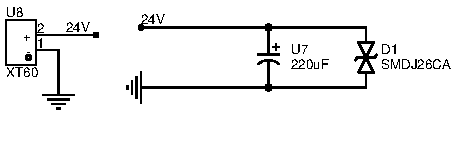
\includegraphics[width=1.3\linewidth]{img/chapter4/huanchong}
					\caption{原理图}
				\end{subfigure}
				\hfill
				\begin{subfigure}{0.45\textwidth}
					\centering
					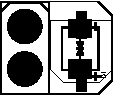
\includegraphics[width=0.7\linewidth]{img/chapter4/huanchongpcb}
					\caption{PCB图}
				\end{subfigure}
				
				\captionsetup{font=scriptsize} 
				\caption{缓冲电路}

			\end{figure}
			为减缓电机启动或断开瞬间可能引发的电气冲击与火花问题,在主电源输入端设计了如图所示的电源缓冲保护电路,该电路主要由滤波电容和瞬态抑制二极管TVS构成。
	\end{frame}
	
	
	
	% Section 5
	\section[软件设计]{软件设计}
	\begin{frame}
		\frametitle{RT-Thread实时操作系统}
		\begin{figure}
			\centering
			\includegraphics[width=0.6\linewidth]{img/chapter5/rtthread}
			\captionsetup{font=scriptsize}
			\caption{RT-Thread软件框架图}
		\end{figure}
		通过不同的线程优先级和控制周期协调运行,实现了系统的并发控制和高实时性。高优先级(如 INS)确保关键数据实时更新;中低优先级线程定期调度,确保控制器与人机交互持续响应
	\end{frame}
		

				

	
	\begin{frame}{线程示例}
		\begin{table}[H]
			\centering
			\caption{线程示例表格}
			\Large
			\begin{tabular}{ccc}
				\toprule
				\textbf{名称} & \textbf{功能} & \textbf{优先级} \\
				\midrule
				INS       & 获取机体姿态                  & 11 \\
				ChassisL  & 左半底盘的运动控制            & 13 \\
				ChassisR  & 右半底盘的运动控制            & 13 \\
				Observe   & 机体运动速度估计,抑制打滑    & 12 \\
				Ps2       & 处理 PS2 手柄传来的遥控数据    & 14 \\
				\bottomrule
			\end{tabular}
		\end{table}
	\end{frame}
	
\begin{frame}
	\frametitle{INS线程}
	
	\begin{minipage}[t]{0.5\linewidth}
		\vspace{-\baselineskip} % 更精确的顶部对齐控制
		\centering
		\includegraphics[width=0.4\linewidth]{img/chapter5/ins} % 图片宽度填满minipage
		\captionof{figure}{INS线程流程图}
	\end{minipage}%
	\hfill % 去掉这行后的空行
	\begin{minipage}[t]{0.4\linewidth}

		\begin{itemize}
			\item \textbf{INS(Inertial Navigation System)}:惯性导航系统线程
			\item 使用Mahony算法获取:
			\begin{itemize}
				\item \textbf{姿态角}(Pitch/Roll/Yaw)
				\item \textbf{绝对加速度}(世界坐标系)
			\end{itemize}
			\item 实时性保障:
			\begin{itemize}
				\item 控制周期:\textbf{1ms}
				\item 线程优先级:\textbf{最高}
			\end{itemize}
		\end{itemize}
	\end{minipage}
\end{frame}
	
	
	\begin{frame}
		\frametitle{姿态解算}

		在三维空间中,可用欧拉角、旋转矩阵、四元数等方式描述刚体姿态:
		
		\begin{itemize}
			\item \textbf{欧拉角}使用三个角度表示刚体绕固定轴的旋转,简洁但存在“万向节死锁”问题。
			\item \textbf{旋转矩阵}是 $3 \times 3$ 的正交矩阵,可通过多个单轴旋转矩阵相乘得到:
			\[
			R = R_x(\theta) R_y(\gamma) R_z(\psi)
			\]
			\[
			R_x(\theta) = \begin{bmatrix}1 & 0 & 0 \\ 0 & \cos\theta & -\sin\theta \\ 0 & \sin\theta & \cos\theta\end{bmatrix}
			\]
			\item \textbf{四元数}通过轴-角形式表示旋转,避免奇异问题,适用于姿态插值和高频更新,计算方便。
		\end{itemize}
	\end{frame}
	
	\begin{frame}{四元数姿态计算方法}
		\small
		四元数极坐标形式为:
		\[
		q = \cos\left(\frac{\theta}{2}\right) + \sin\left(\frac{\theta}{2}\right)(u_x i + u_y j + u_z k)
		\]
		四元数可表示为 $q = q_0 + q_1 i + q_2 j + q_3 k$。其微分形式为:
		\[
		\frac{dq}{dt} = 0.5 \cdot q \otimes \omega
		\]
		其中四元数乘法可写为:
		\[
		Q(q) = \begin{bmatrix}
			q_0 & -q_1 & -q_2 & -q_3 \\
			q_1 & q_0 & -q_3 & q_2 \\
			q_2 & q_3 & q_0 & -q_1 \\
			q_3 & -q_2 & q_1 & q_0
		\end{bmatrix}
		\]
		\[
		\frac{dq}{dt} = 0.5 \cdot Q(q) \begin{bmatrix}0 \\ \omega_x \\ \omega_y \\ \omega_z\end{bmatrix}
		\]
	\end{frame}
	
	\begin{frame}{姿态转换关系}
		\small
		四元数与旋转矩阵之间的转换:
		\[
		R = \begin{bmatrix}
			1-2(q_2^2+q_3^2) & 2(q_1q_2 - q_0q_3) & 2(q_1q_3 + q_0q_2) \\
			2(q_1q_2 + q_0q_3) & 1-2(q_1^2+q_3^2) & 2(q_2q_3 - q_0q_1) \\
			2(q_1q_3 - q_0q_2) & 2(q_2q_3 + q_0q_1) & 1-2(q_1^2+q_2^2)
		\end{bmatrix}
		\]
		
		欧拉角(XYZ顺序)与旋转矩阵转换:
		{\scriptsize
			\[
			R(\alpha, \beta, \gamma) = \begin{bmatrix}
				\cos\beta\cos\gamma & \cos\gamma\sin\alpha\sin\beta - \cos\alpha\sin\gamma & \sin\alpha\sin\gamma + \cos\alpha\cos\gamma\sin\beta \\
				\cos\beta\sin\gamma & \cos\alpha\cos\gamma + \sin\alpha\sin\beta\sin\gamma & \cos\alpha\sin\beta\sin\gamma - \cos\gamma\sin\alpha \\
				-\sin\beta & \cos\beta\sin\alpha & \cos\alpha\cos\beta
			\end{bmatrix}
			\]
		}
		\[
		\left\{
		\begin{aligned}
			\alpha &= \arctan2(R_{32}, R_{33}) \\
			\beta &= -\arcsin(R_{31}) \\
			\gamma &= \arctan2(R_{21}, R_{11})
		\end{aligned}
		\right.
		\]
		微分四元数(角加速度)$\rightarrow$ 四元数(角速度) $\rightarrow$ 旋转矩阵 $\rightarrow$ 欧拉角
		
	\end{frame}
	
	\begin{frame}{姿态角解算中的误差修正}
		\small
		仅依赖陀螺仪角速度积分来估算姿态角会产生累积漂移误差,因此需借助加速度计进行修正:
		
		
		\vspace{0.2cm}
		设定两个重力加速度向量:
		\[
		\mathbf{a} = \begin{bmatrix} a_x \\ a_y \\ a_z \end{bmatrix} \quad
		\mathbf{g} = \begin{bmatrix} g_x \\ g_y \\ g_z \end{bmatrix}
		\]
		将其单位化后进行叉乘,得到误差向量:
		\[
		\mathbf{e} = \mathbf{a} \times \mathbf{g} \approx \sin(\theta) \approx \theta
		\]
		
		\vspace{0.2cm}
		为实现修正:
		\begin{itemize}
			\item 通过误差向量 $\mathbf{e}$ 反映当前角速度积分的偏差。
			\item 引入 PI 控制器,融合加速度计的低频信息,修正角速度漂移,实现互补滤波。
			\item 再用修正后的角速度进行姿态更新,提高稳定性与准确性。
		\end{itemize}
	\end{frame}
	
	
	\begin{frame}
		\frametitle{Observe线程}
			\begin{minipage}[t]{0.5\linewidth}
			\vspace{-\baselineskip} % 更精确的顶部对齐控制
			\centering
			\includegraphics[width=0.25\linewidth]{img/chapter5/kalman.pdf} % 图片宽度填满minipage
			\captionof{figure}{卡尔曼滤波器流程图}
		\end{minipage}%
		\hfill % 去掉这行后的空行
		\begin{minipage}[t]{0.4\linewidth}
			\begin{itemize}
				\item \textbf{Observe}:状态估计线程
				\item 使用卡尔曼滤波算法获取:\textbf{绝对速度}(世界坐标系),抑制机体打滑

				\item 实时性保障:
				\begin{itemize}
					\item 控制周期:\textbf{1ms}
					\item 线程优先级:\textbf{较高}
				\end{itemize}
			\end{itemize}
		\end{minipage}
		
		
	\end{frame}
	
	\begin{frame}{卡尔曼滤波设计}
		\small
		
		\textbf{1. 状态定义}
		{\scriptsize
		定义状态向量:
		\[
		x = \begin{bmatrix} v \\ a \end{bmatrix}
		\]
		
		\textbf{2. 状态方程(匀加速模型)}
		\[
		x_k = F x_{k-1} + w_k, \quad F = \begin{bmatrix} 1 & \delta t \\ 0 & 1 \end{bmatrix}, \quad \delta t = 0.003s
		\]
		过程噪声 $w_k \sim \mathcal{N}(0, Q)$,其中:
		\[
		Q = \begin{bmatrix} 0.5 & 0 \\ 0 & 0.5 \end{bmatrix}
		\]
		
		\textbf{3. 观测方程}
		
		\[
		z_k = H x_k + v_k, \quad z_k = \begin{bmatrix} v_{meas} \\ a_{imu} \end{bmatrix}, \quad H = I
		\]
		观测噪声 $v_k \sim \mathcal{N}(0, R)$,其中:
		\[
		R = \begin{bmatrix} 100 & 0 \\ 0 & 100 \end{bmatrix}
		\]}
		
	\end{frame}
	
	\begin{frame}{卡尔曼滤波五步法}
		\small
		
		\textbf{1. 状态预测}
		\[
		\hat{x}_k^- = F \hat{x}_{k-1}
		\]
		利用上一时刻状态预测当前状态。
		
		\textbf{2. 协方差预测}
		\[
		P_k^- = F P_{k-1} F^T + Q
		\]
		更新预测误差协方差,反映不确定性。
		
		\textbf{3. 卡尔曼增益计算}
		\[
		K_k = P_k^- H^T (H P_k^- H^T + R)^{-1}
		\]

		$R$ 大 → 观测不可靠,$K_k$ 小 → 更信任预测;
		$Q$ 大 → 模型不可靠,$K_k$ 大 → 更信任观测。

		
		\textbf{4. 状态更新}
		\[
		\hat{x}_k = \hat{x}_k^- + K_k (z_k - H \hat{x}_k^-)
		\]
		
		\textbf{5. 协方差更新}
		\[
		P_k = (I - K_k H) P_k^-
		\]
		
		
	\end{frame}
	
	
	\begin{frame}
		\frametitle{Chassis线程}
			\begin{minipage}[t]{0.5\linewidth}
			\vspace{-\baselineskip} % 更精确的顶部对齐控制
			\centering
			\includegraphics[width=1.2\linewidth]{img/chapter5/chassis.pdf} % 图片宽度填满minipage
			\captionof{figure}{底盘控制流程图}
		\end{minipage}%
		\hfill % 去掉这行后的空行
		\begin{minipage}[t]{0.4\linewidth}
			\begin{itemize}
				\item \textbf{Chassis}:底盘控制线程
				\item 利用VMC和LQR算法进行底盘控制:
					\begin{itemize}
						\item 离地检测
						\item 跳跃运动
						\item 自起检测
						\item 转向控制
					\end{itemize}
				\item 实时性保障:
				\begin{itemize}
					\item 控制周期:\textbf{3ms}
					\item 线程优先级:\textbf{较低}
				\end{itemize}
			\end{itemize}
		\end{minipage}
	\end{frame}
	
	
	\begin{frame}
		\frametitle{转向控制}
		\begin{figure}
			\centering
			\includegraphics[width=\linewidth]{img/chapter5/pd.pdf}
			\captionsetup{font=scriptsize}
			\vspace{5pt}
			\caption{PD控制流程图}
		\end{figure}
	期望航向角速度$\psi_d$与姿态解算得到的航向角速度估计值$\hat{\psi}$的误差经过PD控制器得到转向力矩输出,并以相反的符号叠加到状态反馈控制T中以得到左右驱动轮电机的期望力矩$T_l,T_r$。
	\end{frame}
	
	
	\begin{frame}
		\frametitle{离地检测}
			\begin{minipage}[t]{0.5\linewidth}
			\vspace{-\baselineskip} % 更精确的顶部对齐控制
			\centering
			\includegraphics[width=0.8\linewidth]{img/chapter5/ground.pdf} % 图片宽度填满minipage
			\captionof{figure}{离地检测示意图}
		\end{minipage}%
		\hfill % 去掉这行后的空行
		\begin{minipage}[t]{0.4\linewidth}
		\vspace{25pt}
		对于驱动轮,有:
		\[
		\begin{aligned}
			F_N - P - m_w g = m_w \ddot{z}_w \\ \\
			P \approx F \cos{\theta} + \frac{T_p \sin{\theta}}{L_0} \\ \\
			\ddot{z}_w = \ddot{z}_M - \ddot{L}_0 \cos{\theta} + 2 \dot{L}_0 \dot{\theta} \sin{\theta} \\ 
			\quad + L_0 \ddot{\theta} \sin{\theta} + L_0 \dot{\theta}^2 \cos{\theta}
		\end{aligned}
		\]

		\end{minipage}
	\end{frame}
	
		\begin{frame}
		\frametitle{Ps2线程}
		\begin{minipage}[t]{0.5\linewidth}
			\vspace{-\baselineskip} % 更精确的顶部对齐控制
			\centering
			\includegraphics[width=1.1\linewidth]{img/chapter5/ps2.pdf} % 图片宽度填满minipage
			\captionof{figure}{ps2手柄控制流程图}
		\end{minipage}%
		\hfill % 去掉这行后的空行
		\begin{minipage}[t]{0.4\linewidth}
			\begin{itemize}
				\item \textbf{ps2}:ps2手柄控制线程
				\item 接受并处理手柄发送的数据:
				\begin{itemize}
					\item 跳跃控制
					\item roll角控制
					\item 腿长控制
					\item 运动控制
				\end{itemize}
				\item 实时性保障:
				\begin{itemize}
					\item 控制周期:\textbf{10ms}
					\item 线程优先级:\textbf{最低}
				\end{itemize}
			\end{itemize}
		\end{minipage}
	\end{frame}


	
	
	% Section 6
	\section[样机搭建与实验结果]{样机搭建与实验结果}
	
	\begin{frame}
		\frametitle{样机实物}
		\begin{figure}
			\centering
			\includegraphics[width=0.5\linewidth]{img/chapter6/model}
			\captionsetup{font=scriptsize}
			\vspace{5pt}
			\caption{样机实物图}
		\end{figure}
	\end{frame}
	
	\begin{frame}
		\frametitle{越障能力测试}
		\begin{figure}
			\centering
			\includegraphics[width=0.9\linewidth]{img/chapter6/1.pdf}
			\captionsetup{font=scriptsize}
			\vspace{5pt}
			\caption{上坡能力测试}
		\end{figure}
	\end{frame}
	
	
		\begin{frame}
		\frametitle{越障能力测试}
		\begin{figure}
			\centering
			\includegraphics[width=0.9\linewidth]{img/chapter6/2.pdf}
			\captionsetup{font=scriptsize}
			\vspace{5pt}
			\caption{过坡能力测试}
		\end{figure}
	\end{frame}
	
	\begin{frame}
		\frametitle{跳跃能力测试}
		\begin{figure}
			\centering
			\includegraphics[width=0.9\linewidth]{img/chapter6/jump.pdf}
			\captionsetup{font=scriptsize}
			\vspace{5pt}
			\caption{跳跃能力测试}
		\end{figure}
	\end{frame}
	
	
	
	
	\begin{frame}
		\frametitle{性能分析}
		\begin{figure}
			\centering
			\includegraphics[width=0.8\linewidth]{img/chapter6/data.pdf}
			\captionsetup{font=scriptsize}
			\caption{运动数据曲线图}
		\end{figure}
		
		令轮足机器人的期望速度分别为0.4m/s,0m/s,-0.4m/s。其中$\theta$是摆杆与竖直方向夹角,$V_{ref}$是期望速度,$V$是机器人当前速度,$\varphi$是机体与水平夹角。
	\end{frame}
	
	\section[总结]{总结}
	\begin{frame}{总结}
		本研究围绕轮足机器人软硬件一体化设计展开,主要工作:
		\begin{itemize}
			\item 硬件设计:基于STM32H723主控,设计电源滤波电路,设计分电板实现电源的有效分配。
			\item 软件设计:依托RT-Thread系统实现多线程任务调度,确保姿态解算、运动控制等功能的实时性。
			\item 算法设计:采用LQR控制实现轮腿倒立摆姿态稳定、
			基于VMC策略将虚拟力映射为关节力矩
		
			\item 功能实现:实现跳跃、自平衡、转向控制等功能
		\end{itemize}
		
	仿真与样机测试表明,机器人可实现0.4m/s移动、15cm越障及±30°姿态稳定控制,满足复杂场景需求。为应急救援、工业巡检等领域的轮足机器人应用提供了底盘运动基础。
	\end{frame}
	
	
	\section{}
	\logo{\pgfuseimage{badge}}
	\begin{frame}{结束语}
		\begin{center}
			\begin{minipage}{1\textwidth}
				\setbeamercolor{mybox}{fg=white, bg=black!50!blue}
				\begin{beamercolorbox}[wd=0.70\textwidth, rounded=true, shadow=true]{mybox}
					\LARGE \centering 感谢您的聆听!
				\end{beamercolorbox}
			\end{minipage}

		\end{center}
	\end{frame}
	

\end{document}